\section{Quantum Communication System}
    \begin{figure}[tbp]
        \begin{center}
            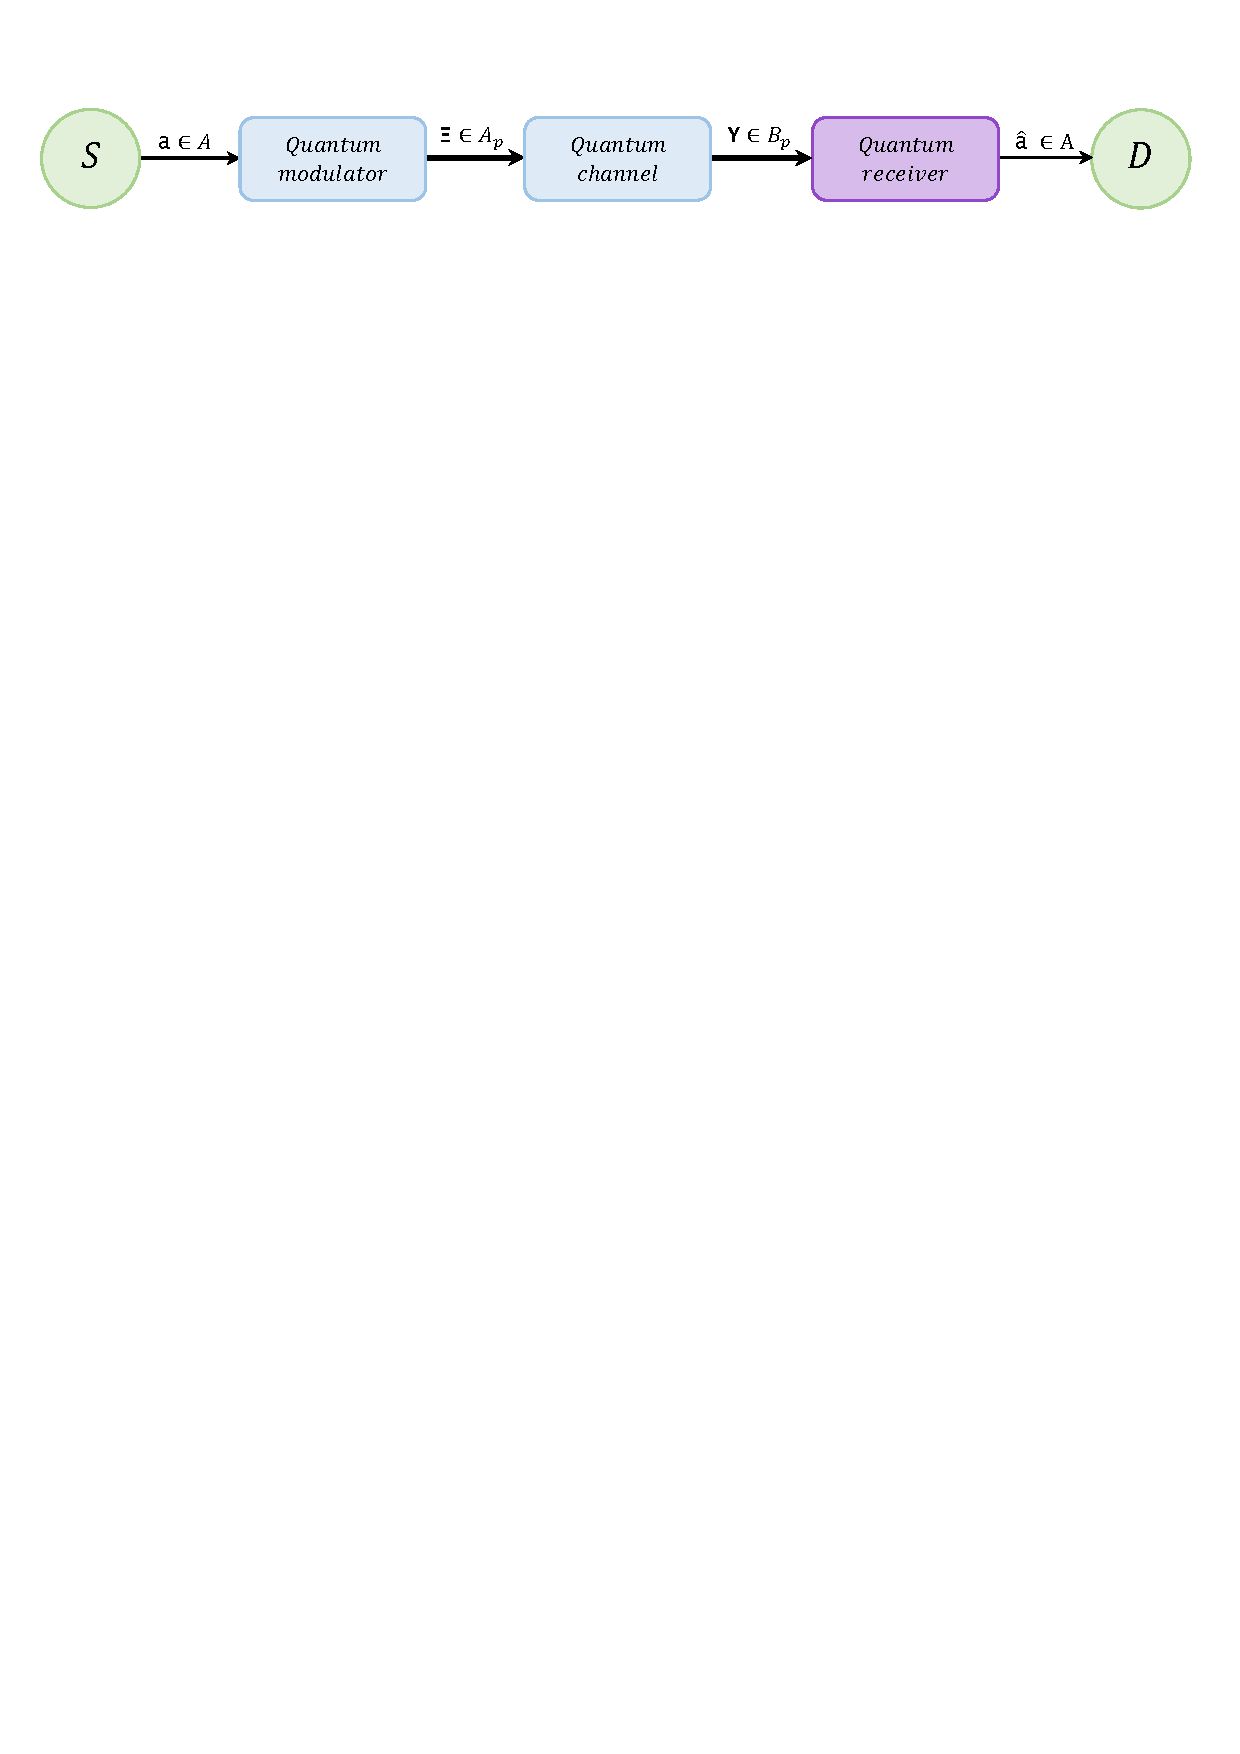
\includegraphics[width=1\textwidth]{fig3.0.pdf}
            \caption{Block-chain of a quantum communication system}
            \label{fig:3.0}
        \end{center}
    \end{figure}
    A quantum communication system can be described similarly to a classical one, as we can 
    see in figure \ref{fig:3.0}. An information source emits a flow symbols $a \in A$, this
    can be considered, without loss of generality, as a flow of bits. These bits have to be 
    modulated with a quantum modulator that emits on the communication channel a quantum state
    $\pmb{\Xi} \in A_p$ for each bit or group of bits. The channel can distort the state and deliver
    the state $\pmb{\Upsilon} \in B_p$ that is in general different from $\pmb{\Xi}$.
    The receiver have to recognize the information $\hat{a}$ as well as possible, i.e. with 
    the minimum possible error probability.
